 \documentclass{article}

\usepackage{bbm}
\usepackage{float}
\usepackage[english]{babel}
\usepackage[utf8]{inputenc}
\usepackage{amsmath}
\usepackage{amsfonts}
\usepackage{algorithm}
\usepackage{algpseudocode}
\usepackage{graphicx}
\usepackage{mwe}    % loads »blindtext« and »graphicx«
\usepackage{subfig}
\usepackage[strict]{changepage}
\DeclareMathOperator*{\argmin}{argmin}

\usepackage{fancyhdr}
\usepackage{subfigure}
\usepackage{float}
\usepackage[utf8]{inputenc}
\usepackage{graphicx}

\begin{document}
\begin{titlepage}
	
	
	\begin{center}
		\vspace{2 cm}
		{\Large \textsc{Francesca Ragusa\\	} }
		{\Large \textsc{Simone Quadrelli} }
	\end{center}
	
	
	\begin{figure}[H]
		\vspace{2 cm}
		\centering
		
\includegraphics[width=0.30\linewidth]{tesiSCIENZE_TECNOLOGIE.jpg}
		
	\end{figure}
	
	\begin{center}
		\vspace{2 cm}
		{\Large \textsc{News categorization with Pegasos} }
	\end{center}

	\par
	\vspace{3 cm}
	
	\begin{center}
		{\large Academic year 2018 - 2019}
	\end{center}
\end{titlepage}



 \pagenumbering{gobble}
\newpage 
\pagenumbering{roman}
\tableofcontents
\listofalgorithms
\listoftables
\listoffigures
\newpage

\pagenumbering{arabic}
\section*{Introduction}
The aim of this work is to compare the performance of two algorithms: Pegasos and Perceptron accoring to their precision and training time on binary classification.\\
Pegasos and Perceptron are supervised learning algorithms, whose output is a vector orthogonal to a uniquely-defined separating hyperplane. This hyperplane divides the space of the datapoints into two half-spaces. The points in the positive half-space, which is the half-space the vector points to, are classified as positives and the others as negatives. The algorithms ideally return the vector that misclassifies the smallest number of datapoints; still some misclassification occurs because datapoints may not be linearly separable.
As expected, Pegasos has better classification performance than Perceptron, however both algorithms provide remarkably good predictors. \\
Both Pegasos and Percepron run efficiently, but Pegasos is approximately three times slower than Perceptron. They both follow a linear growth in the number of epochs. \\
Section \ref{Perceptron} and \ref{Pegaos} provide the description of the algorithms as well as a brief overview of Gradient Descent technique, while section \ref{Dataset} introduces the dataset to the reader.
Section \ref{Pegasos tuning} describes the tuning of the parameter of Pegesos and section \ref{tuning time section} analyzes the execution time of the tuning procedure. Section \ref{Comparison} shows how the comparison between the two algorithms is performed. In section \ref{Results} we show and discuss the results of the experiments.
In the last section we draw the conclusions and comment on the best configuration we suggest to choose.

\newpage
\section{Perceptron} \label{Perceptron}
Perceptron is a learning algorithm used to compute the best separating hyperplane represented by an orthogonal vector $\textbf{w} \mbox{*}$\footnote{In the following we refer to $\textbf{w}$ as separating hyperplane for simplicity} solving to the following problem concerning linearly separable data:
\begin{equation}
\begin{split}
   &   \textbf{w} \mbox{*} = \argmin_{\textbf{w} \in \mathcal{R}^d} \textbf{w} \\
   & s.t.\; y_t\textbf{w}^{T}\textbf{x}_t > 0 \; \forall t \in \{1, ...,m\} 
\end{split}
\end{equation}
\noindent where $\textbf{x} \in \mathcal{R}^d$ is the features vector and $y \in \{-1,1 \}$ is the label of the datapoint.
This hyperplane can be later used to assign a binary label $y=f(\textbf{x})$ to a datapoint $\textbf{x}$, accordingly to:

\begin{equation}
    f(x) = \begin{cases}
                \;\;\;1 & $\textbf{w}\mbox{*} ^T \textbf{x} \geq 0$\\
                -1 & otherwise \\
                \end{cases}
\end{equation}

\noindent When data are linearly separable, Perceptron is guaranteed to converge to an hyperplane that correctly classifies all data. When non-linearly separable data are involved, Perceptron converges to the hyperplane that misclassifies the lowest number of examples. In both cases as the number of examples grows the hyperplane computed approaches to the best possible hyperplane (i.e. the hyperplane with the lowest loss). Unfortunately data are hardly linearly separable, consequently a suitable variation of Perceptron was implemented to handle such a problem. 
\begin{algorithm} [H] \label{perceptron algorithm}
   \caption{Perceptron}
    \begin{algorithmic}[1]
        \State \textbf{inputs}: 
        \State  $ S = \{(\textbf{x}_1,y_1), ..., (\textbf{x}_m,y_m) \}$  \Comment{Set of examples}
        \State T \Comment{number of epochs}
        \State \textbf{initialization:} 
        \State $\textbf{w} = \textbf{0}$ \Comment{accumulator}
        \State $\textbf{w}_0 = \textbf{0}$ \Comment{starting hyperplane}
 		\ForAll{$ t = 1, ..., T$ } 
 			\State $Z_t = random\_uniform(1,m)$ \Comment{extract an index $Z_t \in [1,m]$}
 			\If{$y_{Z_t}\textbf{w}_t^T\textbf{x}_{Z_t} \leq 0$}
 				\State $\textbf{w}_{t+1} = \textbf{w}_t + y_{Z_t}\textbf{x}_{Z_t}$
 			\Else
 			    \State $\textbf{w}_{t+1} = \textbf{w}_t$
 			\EndIf
 		\State $\textbf{w} = \textbf{w} + \textbf{w}_{t+1}$
 		\EndFor
 \State \textbf{return}:  $\frac{\textbf{w}}{T}$
\end{algorithmic}
\end{algorithm}
\noindent 
The best separating hyperplane $\textbf{w} \mbox{*}$ has the minimum hinge loss $$h = [1-y_t{\textbf{w}_t}^T \textbf{x}_t]_+$$ hence to minimize it we exploited Stochastic Gradient Descent (SDG). Stochastic Gradient Descent is a local optimization technique to locate stationary points that is suitable for convex optimization. Indeed, it is a stochastic technique since the data points used to compute the gradient are drawn from a distribution. To ease the analysis datapoints are drawn independently.
In our implementation of Perceptron the stochastic component consists in sampling indices $Z_t$ of the examples from a uniform distribution $[1,m] \subset  \mathcal{N_+}$.
At each iteration of the algorithm, the parameter $\textbf{w}$ is updated accordingly to the gradient of the loss function\footnote{Descending the gradient means to move $\textbf{w}$ toward the direction of the minimum of the loss function. The gradient of the hinge loss is piecewise constant} via:
\begin{equation}
    \textbf{w}_{t+1} = \textbf{w}_t + y_t \textbf{x}_t \mathbbm{1}\{y_t \textbf{w}_t^T \textbf{x}_t \leq 0\}
\end{equation}
\noindent The loss function $h$ is convex, therefore the stationary point found is a minimum. Convexity guarantees that the local minimum is also a global minimum. Hence, SGD with convex functions finds the global minimum. \\
The output is the average of all the hyperplanes computed by the algorithm.


\section{Pegasos} \label{Pegaos}
 Support Vector Machines (SVM) is a model that determines the separating hyperplane with the maximum margin\footnote{margin(w) = $\min_{t=1,..,m} y_t\textbf{w}^T\textbf{x}_t$} between the closest positive labels and negative labels. The hyperplane found in such a way should reduce the probability of misclassification for points with different labels that are close to one another and close to the hyperplane. Therefore, SVM can be seen as a further development of the Perceptron algorithm.
 On a linearly separable data, the SVM solves the following problem:
\begin{equation}
\begin{split}
   &   \textbf{w} \mbox{*} = \argmin_{\textbf{w} \in \mathcal{R}^d} \frac{1}{2} {\lVert \textbf{w} \rVert}^2 \\
   & s.t.\; y_t\textbf{w}^{T}\textbf{x}_t \geq 1 \; \forall t \in \{1, ...,m\} 
\end{split}
\end{equation}
However data are hardly linearly separable, therefore SVM can be generalized to solve the problem on non-linearly separable data as follows:
\begin{equation}
      \textbf{w} \mbox{*} = \argmin_{\textbf{w} \in \mathcal{R}^d} \bigg( \frac{1}{m}\sum_{t=1}^m h_t(\textbf{w}) + \frac{\lambda}{2} {\lVert \textbf{w} \rVert}^2 \bigg)
\end{equation}
To solve the minimization problem Gradient Descent technique can be applied to the SVM. Thus,
Pegasos exploits SGD technique to compute the solution $ \textbf{w} \mbox{*}$ to the following problem:
\begin{equation} 
    \textbf{w} \mbox{*} = \argmin_{\textbf{w} \in \mathcal{R}^d}\bigg( \frac{1}{m}\sum_{t=1}^m h_{Z_t}(\textbf{w}) + \frac{\lambda}{2} {\lVert \textbf{w}\rVert}^2  \bigg)
\end{equation}
where $\textbf{w}$ is a separating hyperplane,  $Z_t$ is a random variable representing the index of the chosen example, $h$ is the hinge loss and $\frac{\lambda}{2} {\lVert \textbf{w} \rVert}^2$ is a regularization term.

\begin{algorithm} [H]
   \caption{Pegasos}  \label{pegasos algorithm}
    \begin{algorithmic}[1]
        \State \textbf{inputs}: 
        \State  $ S = \{(\textbf{x}_1,y_1), ..., (\textbf{x}_m,y_m) \}$  \Comment{Set of examples}
        \State T \Comment{number of epochs}
        \State $\lambda$
        \State \textbf{initialization:} 
        \State $\textbf{w} = \textbf{0}$ \Comment{accumulator}
        \State $\textbf{w}_0 = \textbf{0}$ \Comment{starting hyperplane}
 		\ForAll{$ t = 1, .., T$ } 
 		\State $\eta_t = \frac{1}{\lambda t}$    \Comment{learning rate}
 			\State $Z_t = random\_uniform(1,m)$ \Comment{extract an index $Z_t \in [1,m]$}
 			\If{$\textbf{w}_t^T\textbf{x}_{Z_t} > 0$}
 				\State $\textbf{w}_{t+1} = \textbf{w}_t - \eta_t(-y_{Z_t} \textbf{x}_{Z_t} + \lambda\textbf{w}_t)$
 			\Else
 				\State $\textbf{w}_{t+1} = \textbf{w}_t - \eta_t\lambda\textbf{w}_t$
 			\EndIf
 		\State $\textbf{w} = \textbf{w} + \textbf{w}_{t+1}$
 		\EndFor
 \State \textbf{return}:  $\frac{\textbf{w}}{T}$
\end{algorithmic}
\end{algorithm}
\noindent Again, the stochastic component consists in sampling indices  $Z_t$ of the examples from a uniform distribution $[1,m] \subset  \mathcal{N_+}$.
At each iteration of the algorithm, the parameter $\textbf{w}$ is updated accordingly to the gradient of the loss function\footnote{The gradient in a point can be interpreted as a linear approximation of the function in the neighbourhood of a point.}, however the learning rate $\eta$ limits the movement along the local linear approximation of the function. It is worth noting that there is no need for the learning rate $\eta$ in the Percetron because the hinge loss is piecewise linear, and its gradient is a proper approximation of the funcion in each piece. On the other hand, the loss function $l_{Z_t}(\textbf{w})$ is not linear, consequently the gradient correctly approximates the function just in the neighbourhood of $\textbf{w}$. \\
The loss function $ l_{Z_t}(\textbf{w}) = h_{Z_t}(\textbf{w}) + \frac{\lambda}{2} {\lVert \textbf{w} \rVert}^2$ is $\lambda$-strongly convex and continuous, therefore the stationary point is a minimum. As previously pointed out, convexity also guarantees that the local minimum is also a global minimum. Hence, SGD with convex functions finds the global minimum.
The output is the average of all the hyperplanes computed by the algorithm.

\section{Dataset} \label{Dataset}
The dataset analyzed is a portion of 20000 examples of newsitems from the Reuters dataset. Each newsitem may have more than one label and each feature is the non-zero relative frequency of a word in the whole corpus. We want to train an instance of both Pegasos and Perceptron for each of the four most frequent labels. Since both algorithms need the labels $y$ to be in the set $\{-1,1\}$ a one-vs-all approach was followed: for each of the four most frequent labels $l$ a vector $\textbf{y} \in \{-1,1\}^{20000}$ was defined:
\begin{equation}
   \forall i \in \{1,20000\} \;\;\; y_i = \begin{cases}
                \; \;\,1 & $if i-th newsitem has the label $l$ $\\
                -1 & $otherwise$ \\
                \end{cases}
\end{equation}
There is a feature for each of the 95281 words in the corpus, but for efficiency reasons only non-zero frequencies were saved. Therefore, all the values of the features for each newsitem ($20000 \times 95281$) were saved in a sparse matrix $\textbf{X}$. To store $\textbf{X}$, we used the numpy implementation of sparse matrices because they have small memory footprint and support efficient vector operations.

\section{Pegasos: tuning of $\lambda$} \label{Pegasos tuning}
As a start, we chose some $\lambda$s that span over a wide range of values: $$lbs = \{0.0005, 0.0001, 0.005, 0.001, 0.05, 0.01, 0.05, 0.1, 0.5, 1, 5, 10\}$$The set of possible number of epochs chosen is: $$n\_epochs = \{2000, 3000, 4000, 5000, 6000, 7000, 8000\}$$ It is worth noticing that we chose those values to understand if the classifier generated with few examples is reasonably precise. The number of examples fed to the algorithm in each training phase is 12000. Thus, we decided to limit the number of epoch to values reasonably smaller than the number of examples when tuning the parameter $\lambda$. This choice is also justified by the remarkable computational time needed to tune $\lambda$ for each possible epoch.
\\
Bearing in mind that we want to analyze the performance of the algorithm when T varies, we decided to use as tuned $\lambda$ the one such that:
\begin{equation}
    \lambda = \argmin_{\lambda \in lbs} \bigg(\frac{1}{|n\_epochs|} \sum_{T \in n\_epochs} error(\lambda,T) \bigg)
\end{equation}
where $error$ computes the relative number of misclassified examples by the predictor generated by Pegasos with parameters $\lambda$ and $T$.
The number of epochs in both Pegosos and Perceptron is a parameter of the optimizer (gradient descent) that can influence the precision of the predictors when $\lambda$ is fixed. Therefore we believed reasonable to optimize $\lambda$ for each of the possible values of $T$ in the set $n\_epochs$.\\
To allow the reproducibility of the experiment we set a seed for all the random components of the algorithms. Once the parameters sets are fixed we proceed as follows: the whole dataset is divided in $k=5$ folds, whose elements are randomly extracted. For efficiency reasons, not the data matrix but its indices are divided in folds and are later used to partition the data. This procedure allows to considerably reduce the memory required. \\
The first fold is meant to compute the test error, therefore it is not used to tune $\lambda$. For each number of epochs and for each possible value of $\lambda$ a cross validation is run on the spare folds. Three out of four folds are used to train the model and the remaining one to compute the validation error. The average validation error for each $\lambda$ is then saved.
Once the parameter tuning is over, we chose the $\lambda$ that has the lowest average error with respect to the number of epochs. That $\lambda$ is then used to compute the test error and the four folds exploited for the cross validation are used as training set.
Since there are four most frequent labels, the procedure is repeated four times to find the best $\lambda$ for each label. \\
In the following we provide the pseudocode of the experiment, where the computation of the errors is omitted to highlight the structure of the experiment:
\begin{algorithm} [H]
   \caption{Pegasos tuning}
    \begin{algorithmic}[1]
        \State \textbf{Inputs}: 
        \State  $ D = \{(\textbf{x}_1,y_1), ..., (\textbf{x}_n,y_n) \}$  \Comment{whole dataset}
        \State $k$ \Comment{number of folds }
        \State  $lbs$ \Comment{set of all possible $\lambda$}
        \State $n\_epochs$ \Comment{set of all possible epochs}
        \State \textbf{Tuning procedure}: 
        \State set\_seed \Comment{Allows replication of the experiment}
        \State folds = get\_folds($k$) \Comment{returns the folds}
        \State test\_set = folds[0]\Comment{leave out a fold for testing}
        \State  folds  = folds $ \setminus$ test\_set  \Comment{removing the test fold from the training one}
 		\ForAll{$ T \in  n\_epochs$ } 
 		    \ForAll{$ \lambda \in lbs$ } 
 	            \ForAll{$i \in \{1,..., k-1\}$}  \Comment{run cross validation}
 	                \State validation\_set = folds[i]
 	                \State training\_set = folds $\setminus$ validation\_set
 	                \State  train(training\_set, T, $\lambda$) 
 	            \EndFor
 		    \EndFor
 		\EndFor
 		\State  $\lambda$ =  the  $\lambda$ with the lowest mean validation error
 		\State \textbf{Return:} $\lambda$
\end{algorithmic}
\end{algorithm}
\noindent We did not use the nested cross validation because an external cross validation can approximate the result precisely, while keeping execution time remarkably lower.

\section{Tuning time} \label{tuning time section}
In this section we provide the execution time of the cross validation needed to tune the parameter $\lambda$ for Pegasos; all time measurement relies on a Intel Core i5-7200U dual core processor and 8 GB DDR4 RAM.\\
The total number of pairs ($\lambda$, epoch) tested is 84 for each label. The total number of extracted datapoints used for each labels is:
\begin{equation}
    \sum_{T \in n\_epochs} |lbs| \times T = 420000
\end{equation}
\noindent Overall it amounts to 1680000 extractions.\\ 
As suggested by the plots, the training time is linear in the number of epochs. Furthermore, as the value of $\lambda$ decreases, the training time increases. This is due to the fact that a smaller value of $\lambda$ leads to a greater number of products, since the vector \textbf{w} has more non-zero component. \\
There are no significant difference in the cross-validation execution time among different labels: the time required spans approximately from 15 seconds to 110 seconds per each cross validation.
\begin{figure}[H]
   \begin{adjustwidth}{-4em}{-4em}

     \subfloat{%
       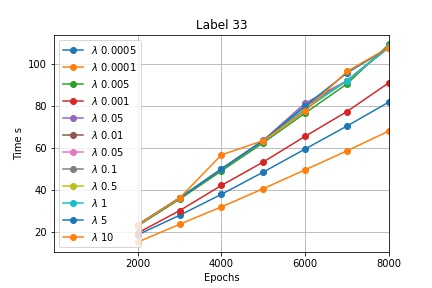
\includegraphics[width=0.60\textwidth]{label1tuning_time.jpg}
     }
     \hfill
     \subfloat{%
       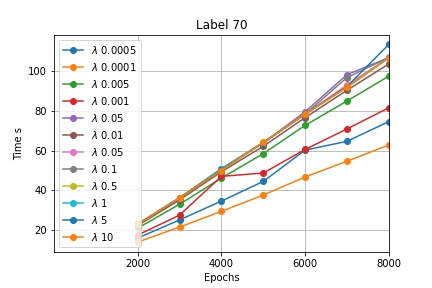
\includegraphics[width=0.60\textwidth]{label2tuning_time.jpg}
     }
     
     \subfloat{%
       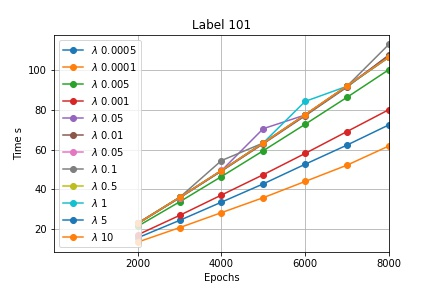
\includegraphics[width=0.60\textwidth]{label3tuning_time.jpg}
     } 
     \hfill
     \subfloat{%
       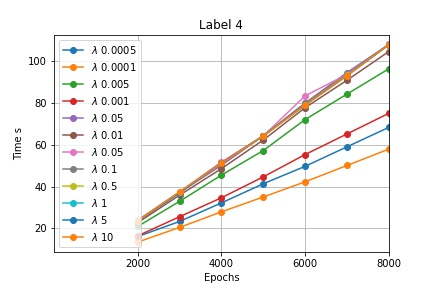
\includegraphics[width=0.60\textwidth]{label4tuning_time.jpg}
     }
     \caption{Tuning time of Pegasos}
     \label{fig: time plot cv}
   \end{adjustwidth}
   \end{figure}
  
\noindent  Overall, the procedure requires about 5 hours and 30 minutes to be completed.

\section{Comparison between Perceptron and Pegasos} \label{Comparison}
As before, this procedure is repeated for each of the four most frequent labels. To simplify the explanation we assume to have fixed the label. \\
We want to compare the performance of both algorithms, given the number of epochs. Even if we used  $n\_epochs$ as the set of epochs in the tuning phase, we will increase up to 20000 the number of iterations in the comparison experiment.
For each number of epochs, Pegasos runs with the optimized $\lambda$ and the training set previously defined, while the Perceptron just exploits the training set. To compare the algorithms we compute the following measures: train error, test error and learning time \footnote{the time required to run the train function}.\\
The pseudocode below provides an insight of the experiment, without the computation of the time required to train the algorithms. 
\begin{algorithm} [H]
   \caption{Perceptron and Pegasos comparison}
    \begin{algorithmic}[1]
     \State \textbf{Inputs}: 
        \State test\_set \Comment{test\_set obtained in the previous experiment}
        \State  $\lambda$ \Comment{tuned $\lambda$}
        \State $n\_epochs$ \Comment{set of all possible epochs}
    \State \textbf{Procedure}: 
	\State  pegasos\_errors = $\emptyset$
	\State  perceptron\_errors = $\emptyset$
 		\ForAll{ $T \in  n\_epochs$}
 	    	\State Pegasos.train(folds, T, $\lambda$) 
 	    	\State pegasos\_errors = pegasos\_errors $\cup$ Pegasos.test\_error(test\_set)
     	  	\State Perceptron.train(folds, T, $\lambda$)
 	    	\State  perceptron\_errors = perceptron\_errors $\cup$ Perceptron.test\_error(test\_set)
 	    \EndFor
        \State \textbf{Return}: pegasos\_errors, perceptron\_errors
\end{algorithmic}
\end{algorithm}

\section{Results} \label{Results}
As a start we extracted the four most frequent labels in the dataset to run one-vs-all classification. Table \ref{table labels} stores them:
\begin{table}[H]
\begin{center}
 \begin{tabular}{||c | c |  c | c| c||} 
 \hline label & 33 & 70 & 101 & 4 \\ [0.5ex] 
    \hline
\end{tabular}
\caption{Most frequent labels in the dataset}
\label{table labels}
\end{center}
\end{table}

\noindent Once the four most frequent labels are known, we extracted the tuned $\lambda$ for each one of them.\\
As shown in Table \ref{table lambda}, the values of $\lambda$ chosen after the optimization process are very small. Bearing in mind that the more $\lambda$ grows, the more the components of vector $\textbf{w}$ are shrunk toward 0. We believe that these values may be suitable for our dataset. Indeed, the vector $\textbf{w}$ has already many 0 components since the data are very sparse. Hence most of the non-zero values of $\textbf{w}$ are required to predict correctly the labels.
\begin{table}[h]
\begin{center}
 \begin{tabular}{||c | c |  c | c| c||} 
 \hline label & 33 & 70 & 101 & 4 \\ [0.5ex] 
    \hline\
   optimal $\lambda$ & 0.0005 & 0.0005  & 0.0005  & 0.0001  \\
 \hline 
\end{tabular}
\caption{Table of the optimal $\lambda$s}
\label{table lambda}
\end{center}
\end{table}


\subsection{Error curves}
In this section we provide an analysis of the error curves as functions of the number of epochs.\\
Pegasos outperforms Pecreptron in classifying the labels 33, 70, 4. Indeed, for each epochs the test error curve of Pegasos lies below the test error curve of Perceptron. However, Perceptron performs slightly better than Pegasos in classifying label 101, right after the number of epochs has reached 14000. \\
Perceptron seems to suffer from a slight overfitting since the distance between training error curve and test error curve increases as the number of epochs grows. Even if in absolute terms the errors are small, the Perceptron test error is twice as big as its train error. On the other hand, Pegasos seems to be more stable: train and test error curves have the same trend and their distance does not change too much.
As the plots below show, the train error and the test error of Pegasos instances are rather stable after 8000 iterations.
\\ Therefore we suggest not to use a number of epochs greater the 8000 when training the model.
\begin{figure}[H]
\begin{adjustwidth}{-4em}{-4em}

     \subfloat{%
       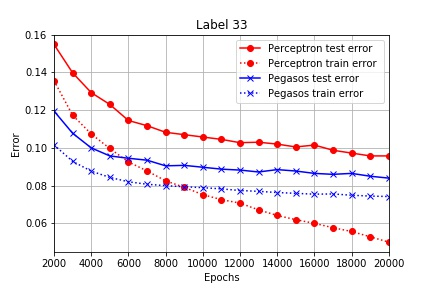
\includegraphics[width=0.60\textwidth]{label1.jpg}
     }
     \hfill
     \subfloat{%
       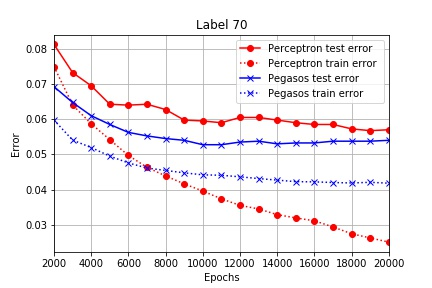
\includegraphics[width=0.60\textwidth]{label2.jpg}
     }
     
     \subfloat{%
       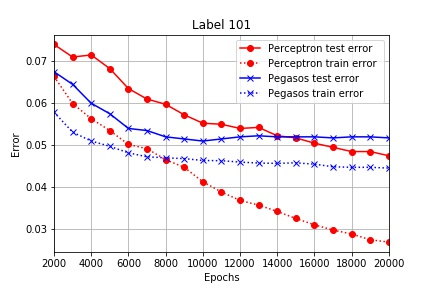
\includegraphics[width=0.60\textwidth]{label3.jpg}
     } 
     \hfill
     \subfloat{%
       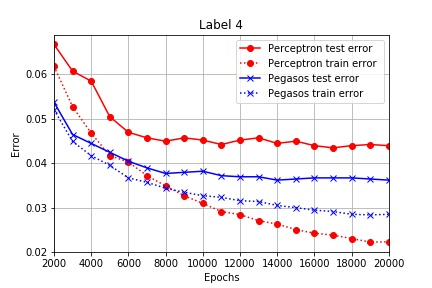
\includegraphics[width=0.60\textwidth]{label4.jpg}
     }
     \caption{The error curves of Percetron and Pegasos.}
     \label{fig:dummy}
    \end{adjustwidth}
   \end{figure}
   
  \subsection{Execution time}
Pegasos update rule requires more scalar products than the update rule of Perceptron, therefore it is reasonable to expect that the execution of the first algorithm needs more time to be completed than the latter.\\
For both the algorithms and for each label the number of updates is linear ($\mathcal{O}(T)$) in the number of epochs T. Notice however that the number of updates may be significantly smaller than T because not all the datapoints generates an update. The time needed to compute the inner products is a small fraction of $\Theta(d)$ \footnote{$d$ is the dimension of $\textbf{w}$}, since the data are very sparse. Therefore the execution time is very low for both algorithms. However, it is possible to notice from the pictures in Figure \ref{time plot} that Pegasos require approximately three times the training time of Perceptron.  Indeed the linear fitting of the execution time points out that the slope of the Percepton curve is approximately 0.001 and the slope of Pegasos is approximately 0.003. This difference is the result of the higher number of products of the Pegasos. 
   \begin{figure}[H]  
   \begin{adjustwidth}{-4em}{-4em}
     \subfloat{%
       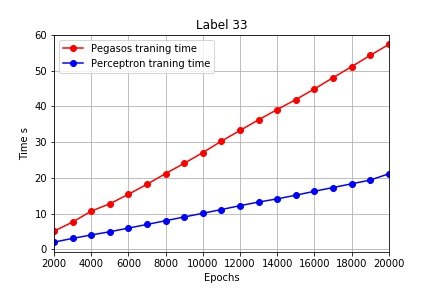
\includegraphics[width=0.60\textwidth]{label1time.jpg}
     }
     \hfill
     \subfloat{%
       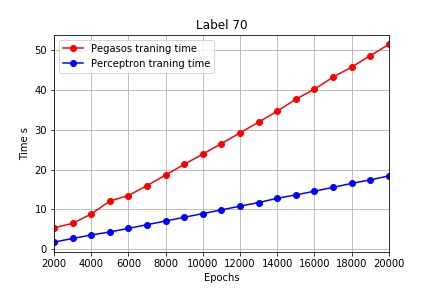
\includegraphics[width=0.60\textwidth]{label2time.jpg}
     }
     
     \subfloat{%
       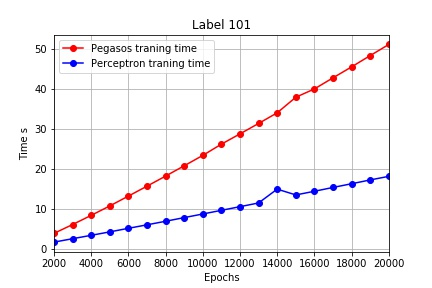
\includegraphics[width=0.60\textwidth]{label3time.jpg}
     } 
     \hfill
     \subfloat{%
       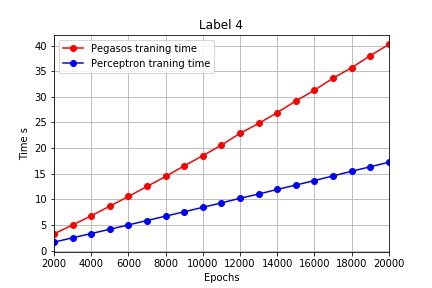
\includegraphics[width=0.60\textwidth]{label4time.jpg}
     }
     \caption{Training time of Perceptron and Pegasos}
     \label{time plot}
   \end{adjustwidth}
   \end{figure}
   
\section{Conclusions} \label{Conclusions}
This work aims to compare the performance of two well-known classification algorithm: Perceptron and Pegasos. 
Theory suggests that Pegasos should have more predictive power and accuracy, despite requiring more training time. In this work we confirmed what theory hinted: overall, Pegasos seems to outperform Pecreptron. Both algorithms reach a remarkable precision, above 90\%.  \\
The execution time of Pegasos is almost three time than the execution time of Perceptron, however there is no point in training Pegasos for more than 8000 epochs because its precision remains stable. Therefore, we suggest to use the predictor computed by Pegasos with 8000 epochs and the tuned $\lambda$ to compute predictions because it is very precise and still requires a very small training time. 

\end{document}